\begin{figure*}[t]
  \centering
    \begin{minipage}[t]{0.48\textwidth}
    \begin{subfigure}[t]{.49\linewidth}
    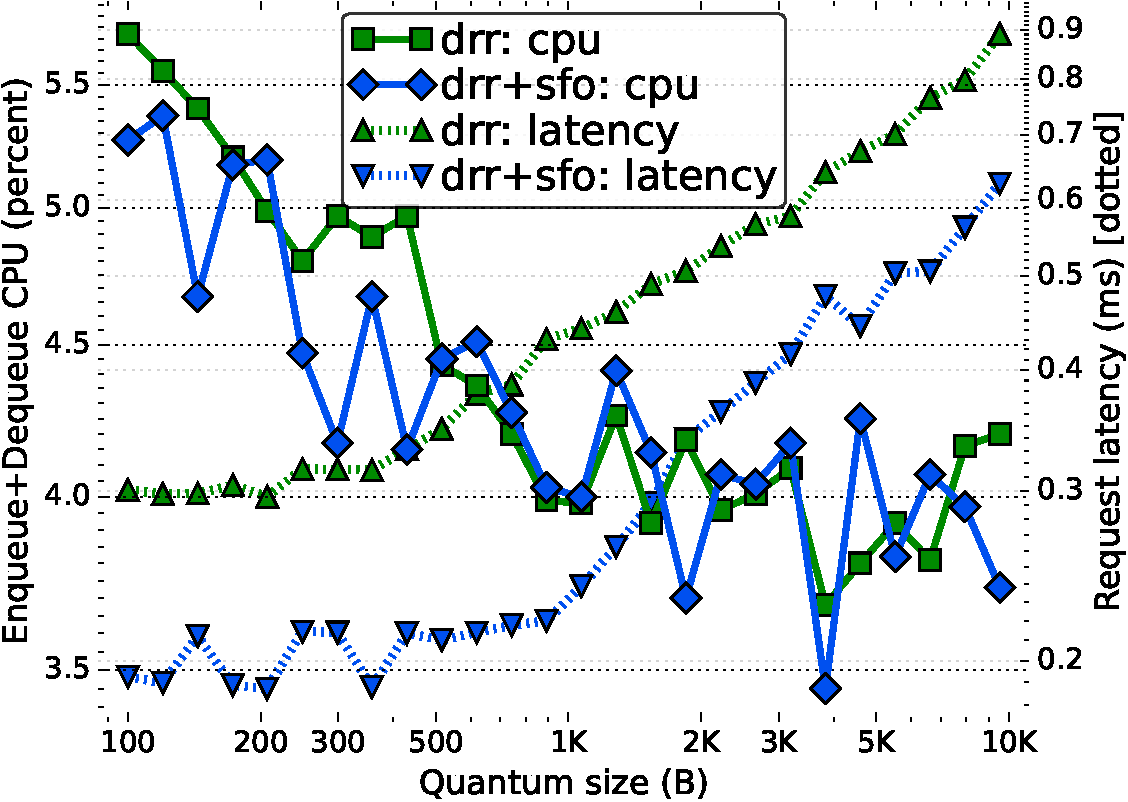
\includegraphics[width=1\linewidth]{figs/burst_cn_2t4x8_mn_2tb2x4_crs_500_kp_lat_drr_basic_fq_drr.pdf}
    \vspace{-6mm}
    \caption{\small{\textit{CPU vs scheduling latency}}}
	\label{fig:quanta-cpu-lat}
    \end{subfigure}
    \begin{subfigure}[t]{.49\linewidth}
        \centering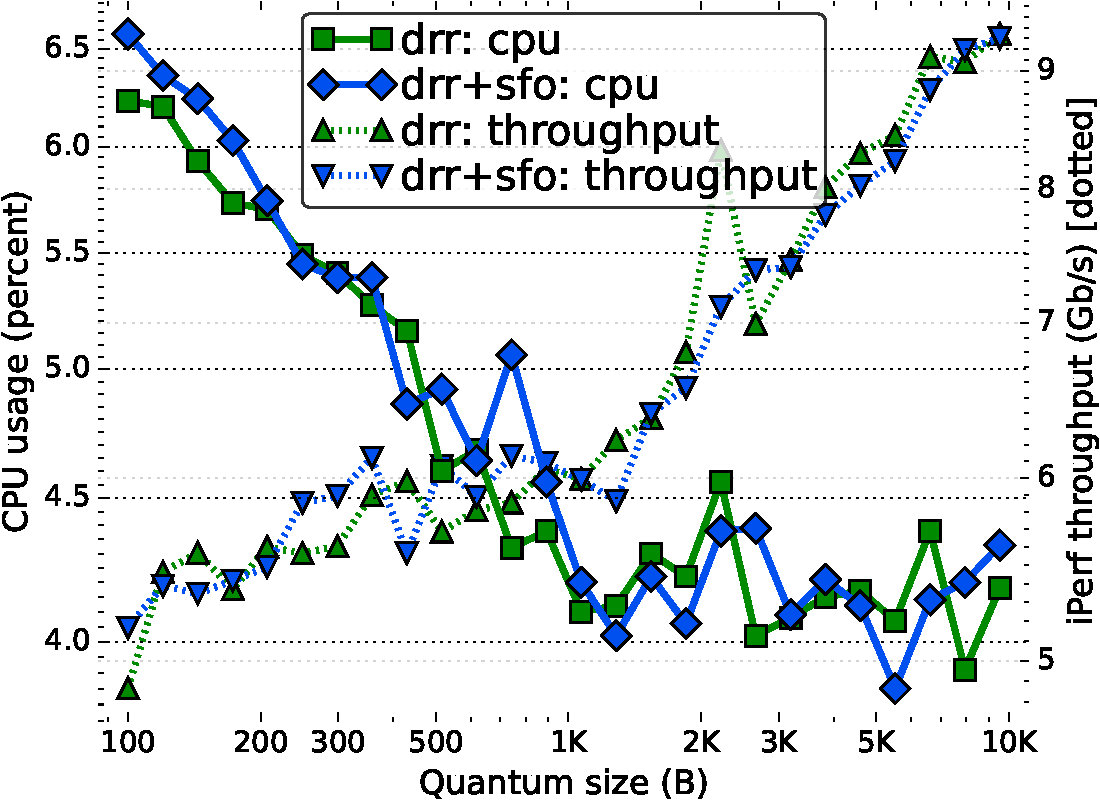
\includegraphics[width=1\linewidth]{figs/burst_cn_6t1x10_mss_1000_kp_bw_drr_basic_fq_drr.pdf}
         \vspace{-6mm}
		\caption{\small{\textit{CPU vs app. throughput}}}
            \label{fig:quanta-cpu-bw}
    \end{subfigure}
        \vspace{-2mm}
    	\caption{\small{
        \textit{Trade-offs in DRR's quantum configuration. }
		}}
	\label{fig:packets}
  \end{minipage}
        \begin{minipage}[t]{0.48\textwidth}
	\centering
	\begin{subfigure}[t]{.49\linewidth}
		\centering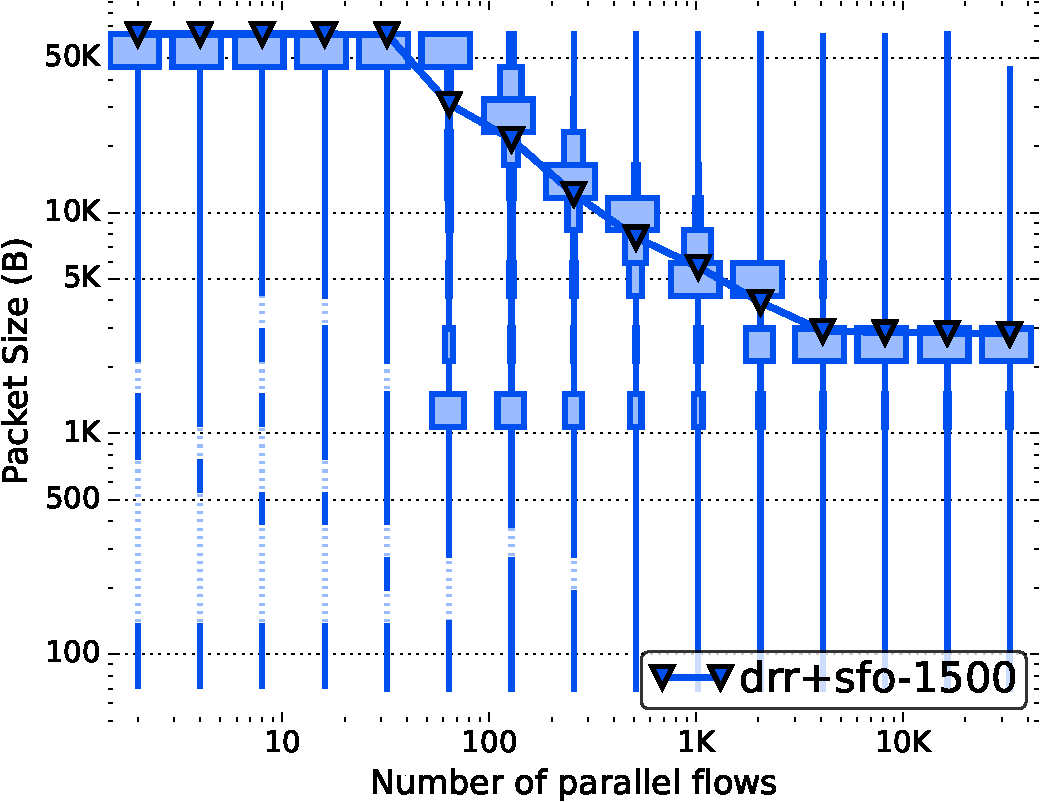
\includegraphics[width=1\linewidth]{figs/paral_cn_1t16x1024_gso_pkthist_fq_drr_1500.pdf}
  \vspace{-6mm}
		\caption{\small{\textit{TSO on TX machine}}}
            \label{fig:packets-edge}
	\end{subfigure}
	\begin{subfigure}[t]{.49\linewidth}
		\centering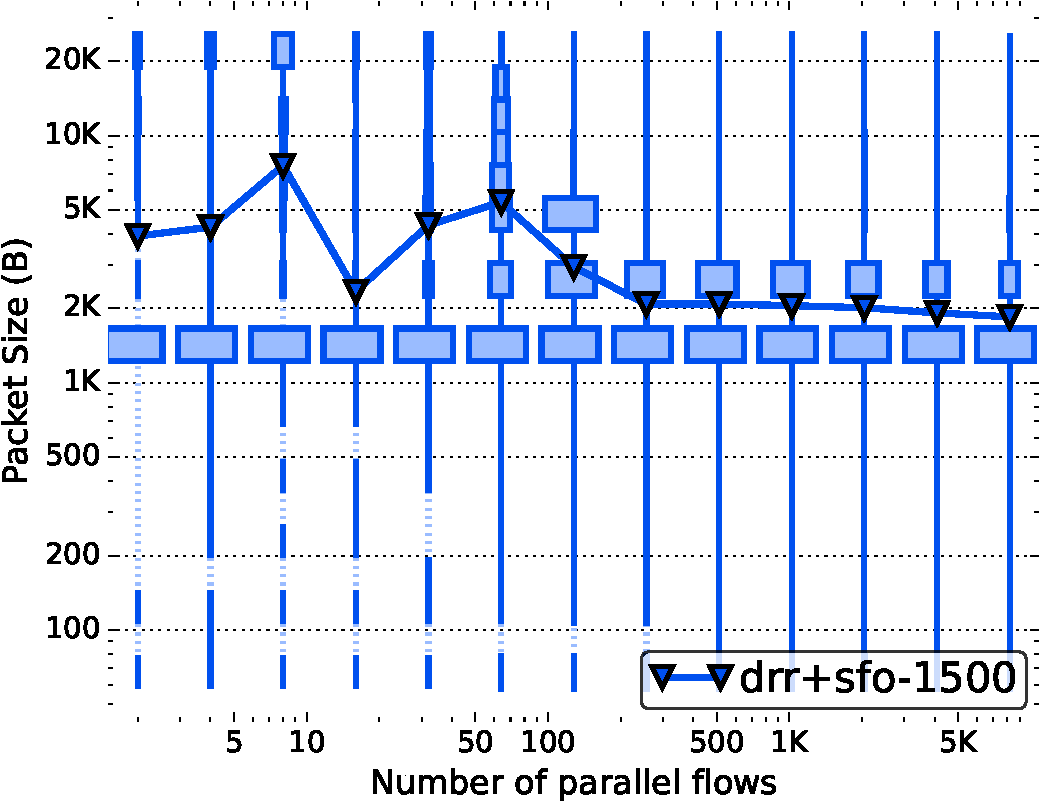
\includegraphics[width=1\linewidth]{figs/paral_cn_1t4x1024_gro_pkthist_fq_drr_1500.pdf}
  \vspace{-6mm}
		\caption{\small{\textit{LRO on RX machine}}}
            \label{fig:packets-core}
	\end{subfigure}
    \vspace{-2mm}
	\caption{\small{
        \textit{SKB length distribution under NIC offloading functions. }
		}}
	\label{fig:packets}
 \end{minipage}
  \vspace{-0.1cm}
\end{figure*}

% \begin{figure}[t]
% 	\centering
% 	\begin{subfigure}[t]{.49\linewidth}
% 		\centering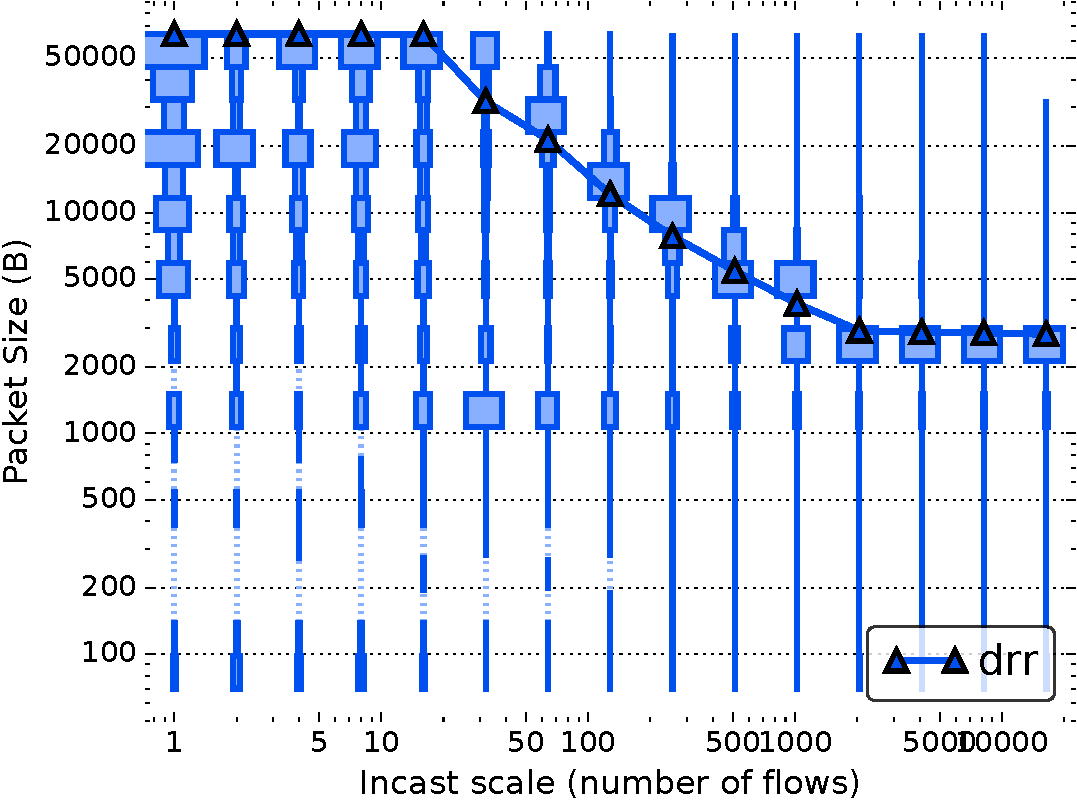
\includegraphics[width=1\linewidth]{figs/paral_pktlength_comp_methods_drr.pdf}
% 		\caption{TSO on TX machine}
%             \label{fig:packets-edge}
% 	\end{subfigure}
% 	\begin{subfigure}[t]{.49\linewidth}
% 		\centering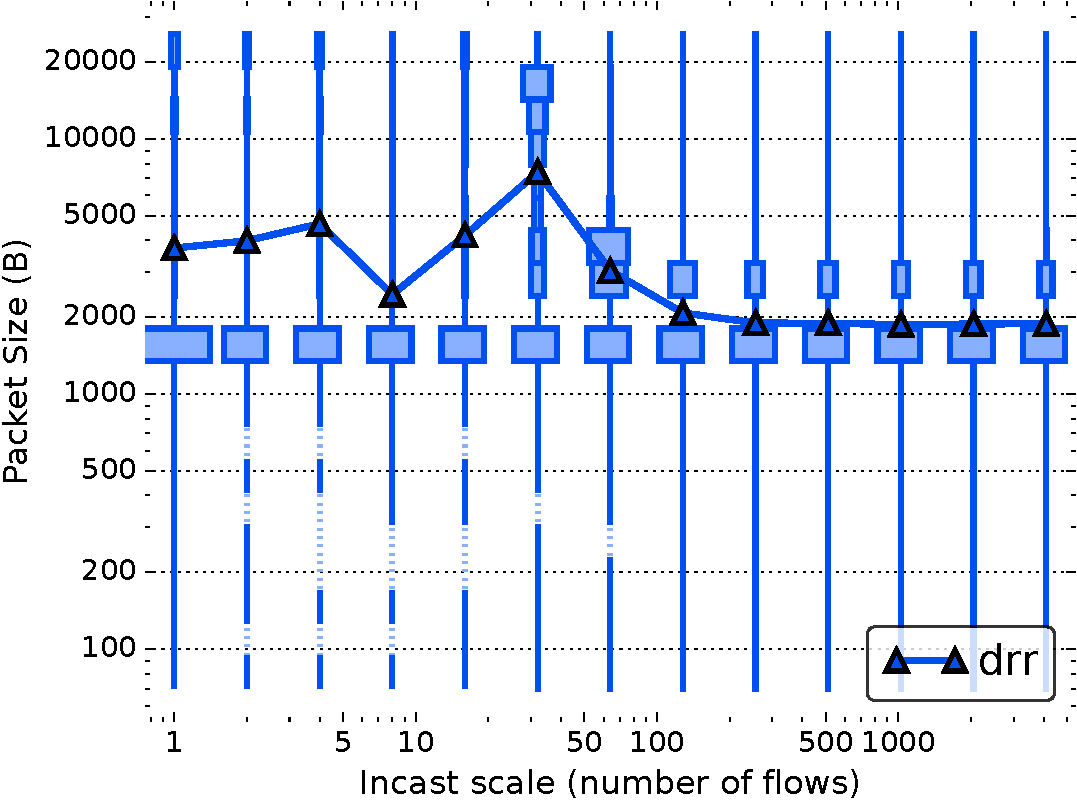
\includegraphics[width=1\linewidth]{figs/paral_pktlength_comp_methods_drr_lro.pdf}
% 		\caption{LRO on RX machine}
%             \label{fig:packets-core}
% 	\end{subfigure}
%     \vspace{-3mm}
% 	\caption{
%         Packet length distribution changes as the number of active TCP flows increases from 1 to 1024 for each connection pair. Enabling the TSO and LRO functionalities drastically widens the possible range of observed packet lengths. The distribution is represented via parallel, independent histogram charts. Wider bins demonstrate higher probability. The straight horizontal line presents the average packet length over different number of parallel flows.
% 		}
% 	\label{fig:packets}
% 	\vspace*{-0.7cm}

% 	\hspace{10pt}
% \end{figure}

